\documentclass[a4paper]{article}

%Пакеты для математических символов:
\usepackage{amsmath} % американское математическое сообщество.
\usepackage{amssymb} % миллион разных значков и готический, ажурный шрифты.
\usepackage{amscd} % диаграммы, графики.
\usepackage{amsthm} % окружения теорем, определений и тд.
\usepackage{physics} % основные физические символы
%\usepackage{latexsym} % треугольники и пьяная стрелка.

%пакеты для шрифтов:
%\usepackage{euscript} % прописной шрифт с завитушками.
\usepackage{MnSymbol} % Значеки доказательства
\usepackage{verbatim} % улучшенный шрифт "пишущей машинки".
%\usepackage{array} % более удобные таблицы.
%\usepackage{multirow} % мультистолбцы в таблицах.
%\usepackage{longtable} % таблицы на несколько страниц.
%\usepackage{latexsym}

\usepackage{etoolbox}
\usepackage{slashbox} %Разделениени текста \backslashbox{}{}
\usepackage{collectbox} % Добавляет коробочки, можно складывать туда текст)


\usepackage{hyperref} % Ссылки как внешние так и внутренние
\hypersetup{
    colorlinks=true,
    linkcolor=black,
    filecolor=magenta,      
    urlcolor=cyan,
    pdftitle={Overleaf Example},
    pdfpagemode=FullScreen,
    }
    
%Пакеты для оформления:
\RequirePackage[center, medium]{titlesec}% Стиль секций и заголовков
%\usepackage[x11names]{xcolor} % 317 новых цветов для текста.
\usepackage{float} % Позволяет использовать H, h! для локации фигур
%\usepackage{multicol} % набор текста в несколько колонн.
\usepackage{graphicx} % расширенные возможности вставки стандартных картинок.
\usepackage{subcaption} % возможность вставлять картинки в строчку
%\usepackage{caption} % возможность подавить нумерацию у caption.
\usepackage{wrapfig} % вставка картинок и таблиц, обтекаемых текстом.
\usepackage{cancel} % значки для сокращения дробей, упрощения, стремления.
\usepackage{misccorr} % в заголовках появляется точка, но при ссылке на них ее нет.
%\usepackage{indentfirst} % отступ у первой строки раздела
%\usepackage{showkeys} % показывает label формул над их номером.
%\usepackage{fancyhdr} % удобное создание верхних и нижних колонтитулов.
%\usepackage{titlesec} % еще одно создание верхних и нижних колонтитулов

%Пакеты шрифтов, кодировок. НЕ МЕНЯТЬ РАСПОЛОЖЕНИЕ.
\usepackage[utf8]{inputenc} % кодировка символов.
%\usepackage{mathtext} % позволяет использовать русские буквы в формулах. НЕСОВМЕСТИМО С tempora.
\usepackage[T1, T2A]{fontenc} % кодировка шрифта.
\usepackage[english, russian]{babel} % доступные языки.

\usepackage{xcolor}
\definecolor{mycolor}{RGB}{244,228,215}

%Отступы и поля:
%размеры страницы А4 11.7x8.3in
\textwidth=7.3in % ширина текста
\textheight=10in % высота текста
\oddsidemargin=-0.5in % левый отступ(базовый 1дюйм + значение)
\topmargin=-0.5in % отступ сверху до колонтитула(базовый 1дюйм + значение)


%Сокращения
%Скобочки
\newcommand{\inrad}[1]{\left( #1 \right)}
\newcommand{\inner}[1]{\left( #1 \right)}
\newcommand{\infig}[1]{\left{ #1 \right}}
\newcommand{\insqr}[1]{\left[ #1 \right]}
\newcommand{\ave}[1]{\left\langle #1 \right\rangle}


%% Красивые <= и >=
\renewcommand{\geq}{\geqslant}
\renewcommand{\leq}{\leqslant}

%%Значек выполнятся
\newcommand{\per}{\hookrightarrow}

%%Векторная алгебра
\newcommand{\rot}{\text{rot}}
\renewcommand{\div}{\text{div}}
\renewcommand{\grad}{\text{grad}}


%% Более привычные греческие буквы
\renewcommand{\phi}{\varphi}
\renewcommand{\epsilon}{\varepsilon}
\newcommand{\eps}{\varepsilon}
\newcommand{\com}{\mathbb{C}}
\newcommand{\re}{\mathbb{R}}
\newcommand{\nat}{\mathbb{N}}
\newcommand{\stp}{$\filledmedtriangleleft$}
\newcommand{\enp}{$\filledmedsquare$}

\makeatletter
\newcommand{\sqbox}{%
    \collectbox{%
        \@tempdima=\dimexpr\width-\totalheight\relax
        \ifdim\@tempdima<\z@
            \fbox{\hbox{\hspace{-.5\@tempdima}\BOXCONTENT\hspace{-.5\@tempdima}}}%
        \else
            \ht\collectedbox=\dimexpr\ht\collectedbox+.5\@tempdima\relax
            \dp\collectedbox=\dimexpr\dp\collectedbox+.5\@tempdima\relax
            \fbox{\BOXCONTENT}%
        \fi
    }%
}
\makeatother
\newcommand{\mergelines}[2]{
\begin{tabular}{llp{.5\textwidth}}
#1 \\ #2
\end{tabular}
}
\newcommand\tab[1][0.51cm]{\hspace*{#1}}
\newcommand\difh[2]{\frac{\partial #1}{\partial #2}}
\newcommand{\messageforpeople}[1]{HSE Faculty of Physics \ \ HSE Faculty of Physics HSE Faculty of Physics \ \ HSE Faculty of Physics HSE Faculty of Physics \ \ HSE Faculty of Physics HSE Faculty of Physics \ \ HSE Faculty of Physics HSE Faculty of Physics \ \ HSE Faculty of Physics HSE Faculty of Physics \ \ HSE Faculty of Physics HSE Faculty of Physics \ \ HSE Faculty of Physics HSE Faculty of Physics \ \ HSE Faculty of Physics }


\numberwithin{equation}{section}

\begin{document}

\begin{flushright}
    Выполнил:

    Карибджанов Матвей
    
    Группа БФЗ211

    Тема:

    Поле излучения диполя
\end{flushright}
\tableofcontents
\newpagestyle{main}{
\setfootrule{0.4pt}
\setfoot{}{\thepage}{\sectiontitle}}
\pagestyle{main}
\pagecolor{mycolor}



\section{Постановка задач}
\subsection{Линейный осцилятор}
\subsection{Линейный осцилятор}
Рассеяние электромагнитной волны на линйном осциляторе, эту модель 
часто применяют для описания рассения на молекулах воздуха, с последующим 
выводом Реллевского рассеяния. 

Формульно зависимость между неподвижным ядром и оцилирующим элемнтом 
в квадратичном поле (квадратичное поле часто являтся результатом приближения), 
с "силой трения" силой линейно зафисящей от скрости элемента во избежании 
резонанса и бесконечного увелечнения амплитуды колебаний. В итоге получим:
\begin{equation}
    m\ddot r + mk \dot r + m\omega^2 r = f(r)
\end{equation}
Где $f(r)-$ некоторая вынуждающая сила.

В задачe в результате ускоренного движения диполь излучает 
электро-магнитные волны, котрые мы ищем.
\subsection{Вращающийс диполь}
Усливия зади просты, вокруг зряженного цетра с постоянной угловой скростью вращается заряд 
рывный по модулю.



\section{Вывод базовых формул}
\subsection{Монохроматические волны}
В первую очередь надо вспомнить что для ЭМ (электромагнитный) волн 
ур. Максвелла преобразуются в:
\begin{gather}
    \begin{matrix}
        \rot E = -\cfrac{1}{c} \cfrac{\partial H}{\partial t} & div H = 0, \\
        \rot H = \cfrac{1}{c} \cfrac{\partial E}{\partial t} & div E = 0.
    \end{matrix}
\end{gather} 
По определению:
\begin{eqnarray}
    H = \rot A; \ 
    E = -\cfrac{1}{c}\cfrac{\partial A}{\partial t} - \grad \phi .
    \label{eq:fil}
\end{eqnarray} 
Воспользуемся нормировеой Лоренца $\partial_i A^i = 0$, \ref{eq:fil} перейдет в:
\begin{eqnarray}
    H = \rot A; \ E = -\cfrac{1}{c}\cfrac{\partial A}{\partial t}.
\end{eqnarray} 
Учитывая запаздывание потенциала, в следствии чего $A\inner{t - \cfrac{x}{c}}$:
\begin{gather}
    \begin{matrix}
    E = -\cfrac{1}{c} A' ; \\ 
    H = \insqr{\nabla, A} = e_{ijk} \partial_j A^k = 
    e_{ijk} \cfrac{\partial \inner{t - x^m /c}}{\partial x^j}  
    \cfrac{\partial A^k}{\partial \inner{t - x^m /c}} =
    -\cfrac{1}{c}e_{ijk} \delta_{jm} \partial_{m} A^k = 
    -\cfrac{1}{c}\insqr{n, A'},
    \end{matrix}
\end{gather}
где $A'$ обозначает дифф. по $\inner{t - \cfrac{x}{c}}$. 
В итоге мы пришли к уже известному результату, что в 
монохроматических волнах:
\begin{eqnarray}
    H = \insqr{n, E}.
\end{eqnarray} 

\subsection{Запаздывающие потенциалы}
В дали от заряда потенциал равен:
\begin{equation}
    d\phi = \cfrac{d e \inner{t - \cfrac{R}{c}}}{R}
\end{equation}
Где $R$ - растоояния от зарядо до точки где измеряем значение потенциала. 
Интегрирования по зарядам дет нам:
\begin{equation}
    \phi = \int \cfrac{1}{R} \rho\inner{r', t - \cfrac{R}{c}} dV'
    \label{eq:fil_p1}
\end{equation}
В $R $ выражается как $R = r - r'$,  $r' -$ 
вектор от начала координат до заряда, $r -$ 
век. от н.к. до точки измерения. Выражение для 
векторного потенциала плучатся аналогично:
\begin{equation}
    A = \cfrac{1}{c} \int \cfrac{j \inner{r',t - R/c}}{R} dV' 
    \label{eq:fil_p2}
\end{equation}

\subsection{Приближение для запаздывающих потенциалов}
Будем считаь что мы измеряем поля на расстониях $r \gg r'$, 
Такое приближение более чем обоснованно при рассмотрении диполя 
(из его определения). И тогда $R = \abs{r' - r} \approx r - \inner{n,r'}$, 
в данном приближении \ref{eq:fil_p1} и \ref{eq:fil_p2} упростяться:
\begin{equation}
    \phi = \cfrac{1}{r} \int \rho\inner{r', t - \cfrac{r - \inner{n,r'}}{c}} dV'
\end{equation}
Может показаться что $r$ взнаменателе протеворечит тому, 
что написано выше но при разложении можно заметить что получится 
$\cfrac{1}{r - \inner{n,r'}} \approx \cfrac{1}{r} + \cancelto{0}{\cfrac{\inner{n,r'}}{r^2}} + ...$.
Аналогичным образом получим:
\begin{equation}
    A = \cfrac{1}{cr} \int j \inner{r',t - \cfrac{r - \inner{n,r'}}{c}} dV',
\end{equation}
обозначив $t' = t - \cfrac{r - \inner{n,r'}}{c}$, $r = R$,
 а также переходя к дискретному виду получим:
\begin{equation}
    A = \cfrac{1}{cR} \sum j \inner{r',t'} = \cfrac{1}{cR} \sum ev.
\end{equation}

\section{Общее решение для диполя}

Теперь зная что:
\begin{equation}
    A = \cfrac{1}{cR} \sum ev = \cfrac{1}{cR} \dot d.
\end{equation}
Так же не забываем про \ref{eq:H_A} и $E = \insqr{H, n}$, получим:
\begin{eqnarray}
    \begin{matrix}
        H = \cfrac{1}{c^2R}\insqr{\ddot d, n}, \\
        E = \cfrac{1}{c^2R}\insqr{\insqr{\ddot d, n}, n}.
    \end{matrix}
    \label{eq:2.5}
\end{eqnarray}
\begin{figure}[H]
    \centering
    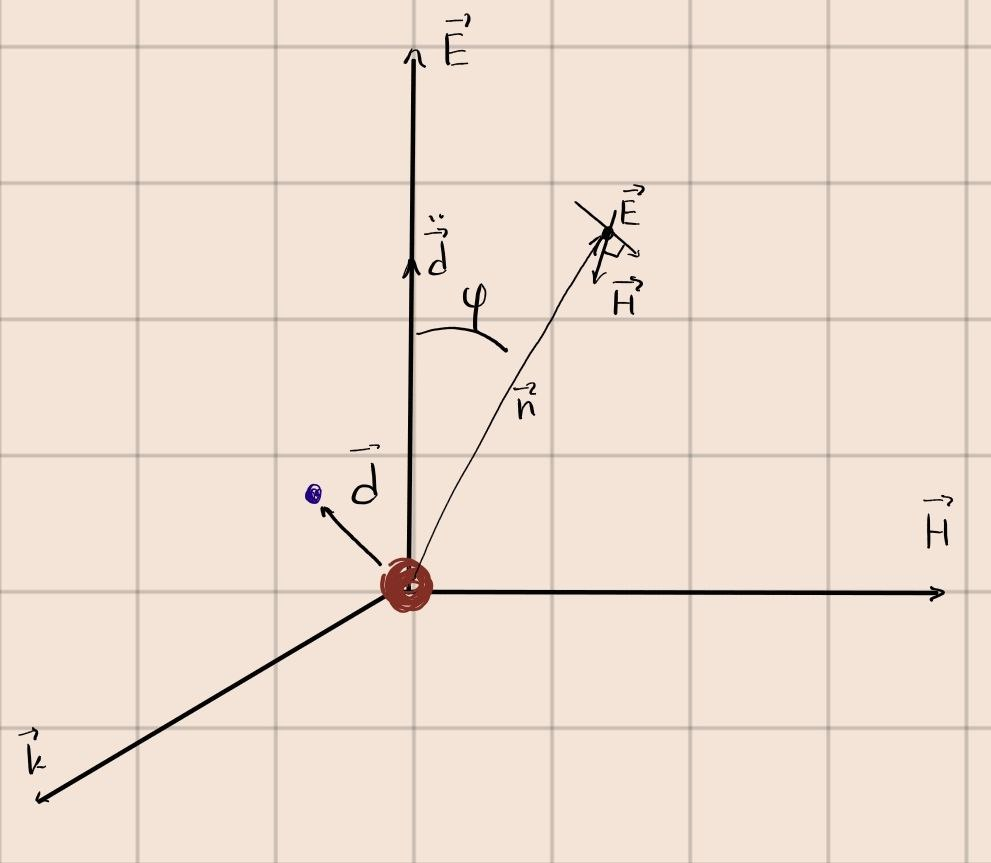
\includegraphics[trim={0 0 0 0},clip,width=\textwidth]{sours_img/sh.jpg}
    \label{pict}
\end{figure}

\subsection{Вектор пойнтинга}
Учитывая ортогональность векторов $H$ и $E$, также то что в 
монохроматической волне $\abs{H} = \abs{E}$, то вектор Пойнтинга
\begin{equation}
    S = \cfrac{cH^2}{4\pi}n.
\end{equation}
От сюда получим 
\begin{equation}
    d\mathfrak{I} = \cfrac{c|H|^2}{4\pi}do
    \label{eq:2.7}
\end{equation}
Подставим $H$ из уравнения \ref{eq:2.5}:
\begin{equation}
    d\mathfrak{I} = \cfrac{c}{4\pi} \cfrac{1}{c^2R} \insqr{\ddot d, n}^2do 
    =  \cfrac{|\ddot d|^2 \sin^2 \phi}{4\pi c^3 R^2} do
    \label{eq:J_ddotd}
\end{equation}


\subsection{Частотное пространство}

Часто удобно работаь в спектральном разложении поэтому посмотрим 
на зависимомти в фурье образа. Напрямую из переобразования формул 
\ref{eq:2.5} получим:
\begin{gather}
    \begin{matrix}
        H_\omega = i \insqr{k, A_\omega},\\
        E_\omega = \cfrac{ic}{\omega} \insqr{k, \insqr{k, A_\omega}},
    \end{matrix}
\end{gather}
Воспользовавшись формулой 
\begin{equation}
    \int_\re f^2 dt = \int_\re \abs{f_\omega}^2 \cfrac{d\omega}{2\pi} 
    = 2\int_{\re_+} \abs{f_\omega}^2 \cfrac{d\omega}{2\pi} 
\end{equation}
Заметив что от в \ref{eq:2.7}  зависит от $t$ только посредстаом $H$ 
получим:
\begin{equation}
    d\mathfrak{I} = \cfrac{c}{2\pi} \abs{H_w}^2R^2do
    \label{eq:if}
\end{equation}
\section{Решение для линейноного осцилятора}
\subsection{Приближения и уточнение формулировки}

Во первых вспомнм что:
\begin{equation}
    p  = \cfrac{mv}{\sqrt{1 - \cfrac{v^2}{c^2}}}.
\end{equation}
В не релятивистком случае уравненнеие сильно упрощается:
\begin{equation}
    p \approx mv,
\end{equation}
поэтому предлагаю решать в приближении $v/c \ll 1$.
Тогда известное нам уравнение:
\begin{equation}
    \cfrac{dp}{dt} = e  E + \cfrac{e}{c} \insqr{ v,  H},
\end{equation}
выродится в: 
\begin{equation}
    m\cfrac{dv}{dt} = e  E.
\end{equation}
От сюда следует что можно пренебречь влиянием магнитного поля на диполь и 
рассматривать только электрическое поле. 

\subsection{Диф. уравнение}
 
Запишем наше уравнение:
\begin{equation}
    m \ddot r + mk\dot r + m\omega_0^2r = e E(t).
\end{equation}
Как уже ясно я предлагаю использовать преобразование фурье для решения:
\begin{equation}
    -\omega^2 r - i\omega kr + \omega_0^2r = \cfrac{e}{m} E_\omega.
\end{equation}
Вспомним что в излучение диполя основной вклад дает компонента $\ddot d$,
А так как так как центральный заряд не подвижен и закреплен в начале СО 
то $d = e r \implies \ddot{d} = e\ddot{{r}}$. Тогда 
нам нужно искать:
\begin{equation}
    r = \cfrac{eE_\omega}{m\inner{\omega_0^2 - i\omega k - \omega^2 }}.
\end{equation}
\begin{equation}
    \mathfrak F \insqr{\ddot d}(\omega)= -e\omega^2 r = 
    -\cfrac{e\omega^2E_\omega}{m\inner{\omega_0^2 - i\omega k 
    - \omega^2 }}.
    \label{eq:ddot_d}
\end{equation}

Получим распределение полей в общем виде, подставив $\ddot d$ в \ref{eq:2.5}:
\begin{equation}
    H = \cfrac{e}{mc^2R}\insqr{\int_\re
    \cfrac{\omega^2E_\omega}{\inner{\omega_0^2 - i\omega k - \omega^2 }}\exp{-it\omega}\cfrac{d\omega}{2\pi}, n},
    \label{eq:fild}
\end{equation}
\begin{equation}
    E = \insqr{H, n}.
\end{equation}
Естественно что поле зависит от висит от времени, и угла измерения, 
в качестве параметров выступают характеристики диполя и падющей волны. 

Если предположить что на диполь падает монохроматическая волна то 

\begin{equation}
    H = \cfrac{e}{mc^2R}\insqr{\int_\re
    \cfrac{\omega^2 E_0 \cancel{2 \pi} \delta (w_v+w) \exp (-ikx)}{\inner{\omega_0^2 - i\omega k - \omega^2 }}\exp{-it\omega}
    \cfrac{d\omega}{\cancel{2 \pi}}, n}
\end{equation}

\begin{equation}
    = \cfrac{e[E_0, n]}{mc^2R}\int_\re
    \cfrac{\omega^2 \delta (w_v-w) \exp (-ikx)}{\inner{\omega_0^2 - i\omega k - \omega^2 }}\exp{-it\omega}
    d\omega = 
    \cfrac{e[E_0, n]}{mc^2R}
    \cfrac{\omega_v^2 \exp (-iw_v t-ikx)}{\inner{\omega_0^2 - i\omega_v k - \omega_v^2 }}
\end{equation}
Мы получили что при падении монохроматической волны на диполь, он испускает 
в ответ монохроматическую волну но с другой амплитудой при этом зависящей от 
угла, угол появлятся из векторно произведения $[E_0, n]$


\subsection{Распределение интенсивности}

Пользуясь формулой \ref{eq:if} получим:
\begin{equation}
    d\mathfrak{I} = \cfrac{1}{4\pi c^3}\insqr{\ddot{d}, n}^2do
    = \cfrac{1}{4\pi c^3}\ddot d^2_\omega \sin^2\phi do.
\end{equation}
Подставляем решение \ref{eq:ddot_d}:
\begin{equation}
    d\mathfrak{I} = \cfrac{1}{4\pi c^3} \abs{\cfrac{eE_\omega}{m\inner{\omega_0^2 
    - i\omega k - \omega^2 }}}^2 \sin^2\phi do.
\end{equation}
Проинтегрируем по всем углам, использовав соотношение $do = 2 \pi \sin{\phi} d\phi$:
\begin{equation}
    \mathfrak{I} = \cfrac{2}{3c^3} \ddot{d}^2_\omega.
\end{equation}

Для падающей монохроматической волны получим:
\begin{equation}
    d\mathfrak{I} =  \cfrac{\inner{eE_0 \sin \theta}^2}{4\pi c^3 \inner{mc^2R}^2} 
    \cfrac{\omega_v^4}{\inner{\omega_0^2 - \omega_v^2 }^2 + \omega_v^2 k^2 } do
\end{equation}
Обозначим $\xi = \cfrac{\inner{eE_0 \sin \theta}^2}{4\pi c^3 \inner{mc^2R}^2}$
\begin{figure}[H]
    \centering
    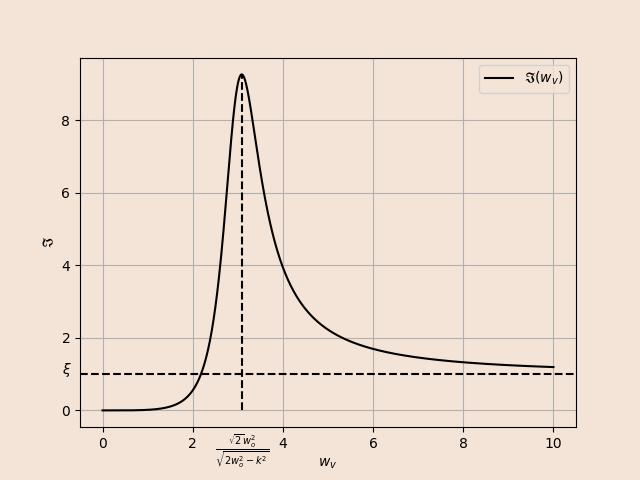
\includegraphics[width=1\textwidth]{sours_img/omega.jpg}
    \caption{Еденицами измерения по оси y выступает $\xi$}
    \label{pict:j_w}
\end{figure}

Как мы видим на грфике прослеживается явный максимум в зависимоти $\mathfrak{I}(w_v)$ 
а то значит, что налетающая волнп попала в резоннас с диполем, такой случай
называют Реллеевским рассеянием. 

\begin{figure}[H]
    \centering
    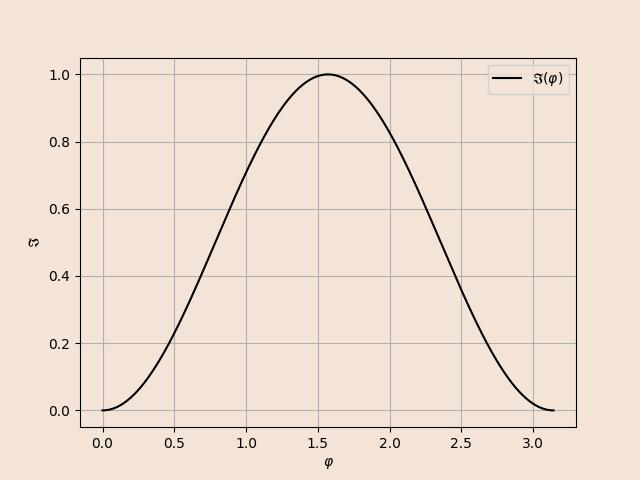
\includegraphics[trim={0 0 0 0},clip,width=1\textwidth]{sours_img/phi.jpg}
    \label{pict:J_phi}
\end{figure}



\section{Вращающийся диполь}
Заметим что задача обладает аксиальной симметрией, поэтому в полярных координата
\begin{eqnarray}
    x &=& r \cos \omega t\\
    y &=& r \sin \omega t
\end{eqnarray}

\begin{gather}
    d = e
    \begin{pmatrix}
        x \\ y
    \end{pmatrix}
    = e
    \begin{pmatrix}
        r\cos \omega t \\ r\sin \omega t
    \end{pmatrix}
    \implies 
    \ddot d =
    \begin{pmatrix}
        -r \omega \sin \omega t \\ r \omega \cos \omega t
    \end{pmatrix}
\end{gather}

Аналогично подставим в \ref{eq:J_ddotd}, получим:
\begin{eqnarray}
    \mathfrak{I} = \cfrac{\omega^2 r^2 e^2 }{4\pi c^3} \sin^2 \phi do
\end{eqnarray}

Поляризацию определим как 














\section{Вывод}

Как мы видим для знания поля нужна информация о параметрах диполя. 
Например для велечины поля по формуле \ref{eq:fild}. Для решении 
не использовались вектора Герца, было очень удобно пользоваться 
формализмом векоторного потенциала.

В общем виде были выведены зависимомти $H(\ddot d)$, доказано что $E \perp H$,
$\mathfrak{I}(\ddot d)$ и тп. Было рассмотрено частотное представление.

Для задачи линейного осцилятора были сделаны приближения по влиянию $E, H$ на 
$d$. Блыли нейдены $H, E$ излучаемые диполем как в общем случе так идля плоской 
монохроматической волны. Была найлена резонанссная частота (смотри график \ref{pict:j_w})
Было надено излечени в телесный угол и полное излечение.

Для вращ. диполя нашли распределение интенсивности в телесны угол и 
поляризацию исппускаемой волны.




\end{document}